\documentclass[12pt, journal]{IEEEtran}

\usepackage{tfrupee}
\usepackage{enumitem}
\usepackage{amsmath}
\usepackage{amssymb}
\usepackage{cite}
\usepackage{amsmath,amssymb,amsfonts,amsthm}
\usepackage{algorithmic}
\usepackage{graphicx}
\usepackage{textcomp}
\usepackage{xcolor}
\usepackage{txfonts}
\usepackage{listings}
\usepackage{enumitem}
\usepackage{mathtools}
\usepackage{gensymb}
\usepackage[breaklinks=true]{hyperref}
\usepackage{tkz-euclide} % loads  TikZ and tkz-base
\usepackage{listings}

\DeclareMathOperator*{\Res}{Res}
%\renewcommand{\baselinestretch}{2}
\renewcommand\thesection{\arabic{section}}
\renewcommand\thesubsection{\thesection.\arabic{subsection}}
\renewcommand\thesubsubsection{\thesubsection.\arabic{subsubsection}}

\renewcommand\thesectiondis{\arabic{section}}
\renewcommand\thesubsectiondis{\thesectiondis.\arabic{subsection}}
\renewcommand\thesubsubsectiondis{\thesubsectiondis.\arabic{subsubsection}}

% correct bad hyphenation here
\hyphenation{op-tical net-works semi-conduc-tor}
\def\inputGnumericTable{}                                 %%

\lstset{
%language=C,
frame=single, 
breaklines=true,
columns=fullflexible
}


\title{Hardware Assignment \\ \Large AI1110: Probability and Random Variables \\ \large Indian Institute of Technology Hyderabad}
\author{Arugonda Srikar \\ \normalsize CS22BTECH11008 \\ \large Random number generators using shift registers}

\begin{document}
	\newtheorem{theorem}{Theorem}[section]
	\newtheorem{problem}{Problem}
	\newtheorem{proposition}{Proposition}[section]
	\newtheorem{lemma}{Lemma}[section]
	\newtheorem{corollary}[theorem]{Corollary}
	\newtheorem{example}{Example}[section]
	\newtheorem{definition}[problem]{Definition}
	%\newtheorem{thm}{Theorem}[section] 
	%\newtheorem{defn}[thm]{Definition}
	%\newtheorem{algorithm}{Algorithm}[section]
	%\newtheorem{cor}{Corollary}
	\newcommand{\BEQA}{\begin{eqnarray}}
	\newcommand{\EEQA}{\end{eqnarray}}
	\newcommand{\define}{\stackrel{\triangle}{=}}

	\bibliographystyle{IEEEtran}
	%\bibliographystyle{ieeetr}


	\providecommand{\mbf}{\mathbf}
	\providecommand{\pr}[1]{\ensuremath{\Pr\left(#1\right)}}
	\providecommand{\qfunc}[1]{\ensuremath{Q\left(#1\right)}}
	\providecommand{\sbrak}[1]{\ensuremath{{}\left[#1\right]}}
	\providecommand{\lsbrak}[1]{\ensuremath{{}\left[#1\right.}}
	\providecommand{\rsbrak}[1]{\ensuremath{{}\left.#1\right]}}
	\providecommand{\brak}[1]{\ensuremath{\left(#1\right)}}
	\providecommand{\lbrak}[1]{\ensuremath{\left(#1\right.}}
	\providecommand{\rbrak}[1]{\ensuremath{\left.#1\right)}}
	\providecommand{\cbrak}[1]{\ensuremath{\left\{#1\right\}}}
	\providecommand{\lcbrak}[1]{\ensuremath{\left\{#1\right.}}
	\providecommand{\rcbrak}[1]{\ensuremath{\left.#1\right\}}}
	\theoremstyle{remark}
	\newtheorem{rem}{Remark}
	\newcommand{\sgn}{\mathop{\mathrm{sgn}}}
	\providecommand{\abs}[1]{\left\vert#1\right\vert}
	\providecommand{\res}[1]{\Res\displaylimits_{#1}} 
	\providecommand{\norm}[1]{\left\lVert#1\right\rVert}
	%\providecommand{\norm}[1]{\lVert#1\rVert}
	\providecommand{\mtx}[1]{\mathbf{#1}}
	\providecommand{\mean}[1]{E\left[ #1 \right]}
	\providecommand{\fourier}{\overset{\mathcal{F}}{ \rightleftharpoons}}
	%\providecommand{\hilbert}{\overset{\mathcal{H}}{ \rightleftharpoons}}
	\providecommand{\system}{\overset{\mathcal{H}}{ \longleftrightarrow}}
	%\newcommand{\solution}[2]{\textbf{Solution:}{#1}}
	\newcommand{\solution}{\noindent \textbf{Solution: }}
	\newcommand{\cosec}{\,\text{cosec}\,}
	\providecommand{\dec}[2]{\ensuremath{\overset{#1}{\underset{#2}{\gtrless}}}}
	\newcommand{\myvec}[1]{\ensuremath{\begin{pmatrix}#1\end{pmatrix}}}
	\newcommand{\mydet}[1]{\ensuremath{\begin{vmatrix}#1\end{vmatrix}}}
	
		\maketitle
	\section*{Components:}
	\begin{table}[htbp]
		\label{tab:Hardware_Assignment}
		%%%%%%%%%%%%%%%%%%%%%%%%%%%%%%%%%%%%%%%%%%%%%%%%%%%%%%%%%%%%%%%%%%%%%%
%%                                                                  %%
%%  This is a LaTeX2e table fragment exported from Gnumeric.        %%
%%                                                                  %%
%%%%%%%%%%%%%%%%%%%%%%%%%%%%%%%%%%%%%%%%%%%%%%%%%%%%%%%%%%%%%%%%%%%%%%
\begin{tabular}{|l|l|l|}\hline
	Component	&Value &Quantity\\ \hline
	Breadboard & &1 \\ \hline
	Seven Segment Diplay &Common Anode &1 \\ \hline
	Decoder &7447 &1 \\ \hline
	Flip Flop &7474 &2 \\ \hline
	X-OR Gate &7486 &1 \\ \hline
	555 IC & &1 \\ \hline
	Resistor &1 K$\Omega$ &1 \\ \hline
	Capacitor &100 nF &1 \\ \hline
	Capacitor &10 nF &1 \\ \hline
	Jumper Wires & & \\ \hline
\end{tabular}

	\end{table}
	\section*{Working Procedure}
	\begin{enumerate}
	\item Connect the 555 timer circuit as shown in fig1. Then the clock signal output is generated. \\\\
	\item The output generated is connected to 3rd and 11th pins of both 7474 IC's. These 7474IC's contains 2 D-flip flops inside them. It is shown in fig2. \\\\
	\item The output of 1st and 4th flipflop is connected to input of XOR gate(7486) as in fig 3 and output of XOR is connected to input of 1st flip flop.\\\\
	\item Connect the Decoder's(7447) A, B, C, D with output of each flip flops($Q_0$, $Q_1$, $Q_2$, $Q_3$) decoder is shown in fig4.\\\\
	\item Then connect the 7-segment display with the decoder. refer fig-5 and fig-6.\\\\
	\end{enumerate}
	\section*{Output}
	7-segment display displays a random number from $0-9$.\\
	\begin{figure}[h]
		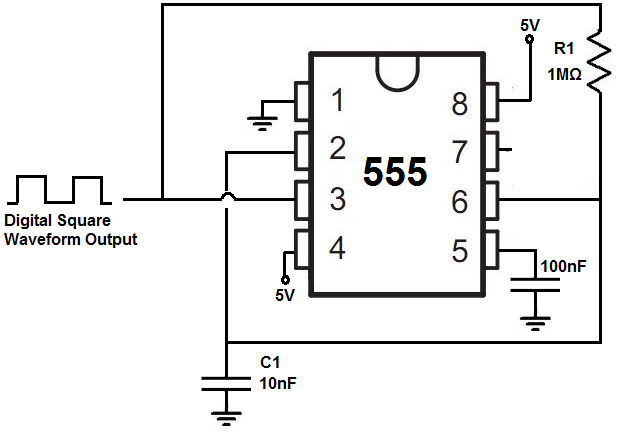
\includegraphics[width=\linewidth]{img/555.png}
		\caption{ 555 timer circuit}
		\label{fig-1}
	\end{figure}
	\begin{figure}[ht]
		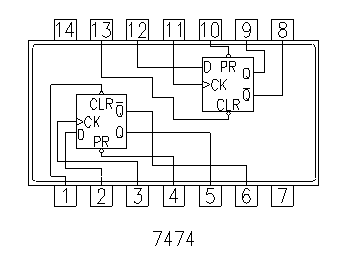
\includegraphics[width=\linewidth]{img/IC7474.png}
		\caption{ 7474 containing 2 D-Flipflops}
		\label{fig-2}
	\end{figure}
	\begin{figure}[ht]
		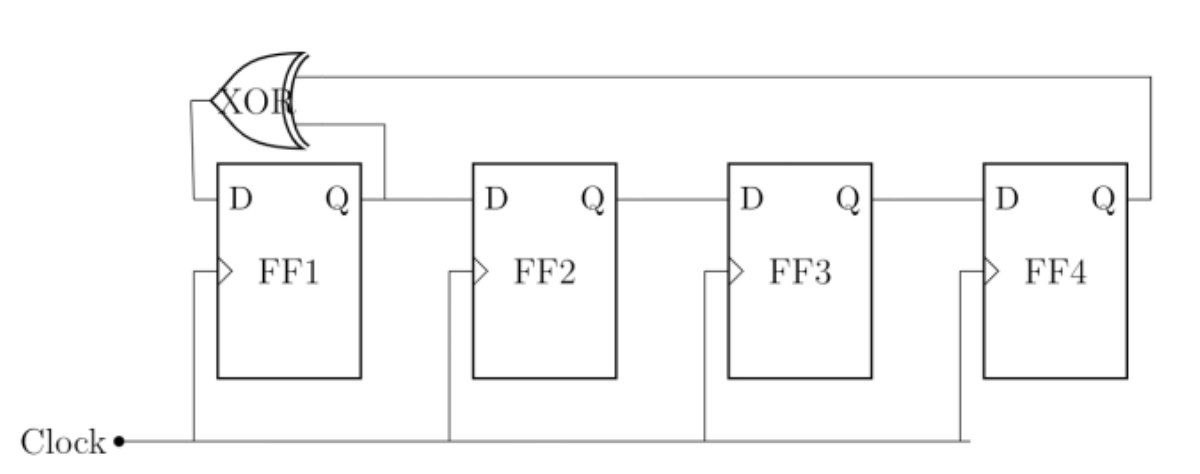
\includegraphics[width=\linewidth]{img/circuit.jpg}
		\caption{ connections between two 7474's and 7486}
		\label{fig-3}
	\end{figure}
	\begin{figure}[ht]
		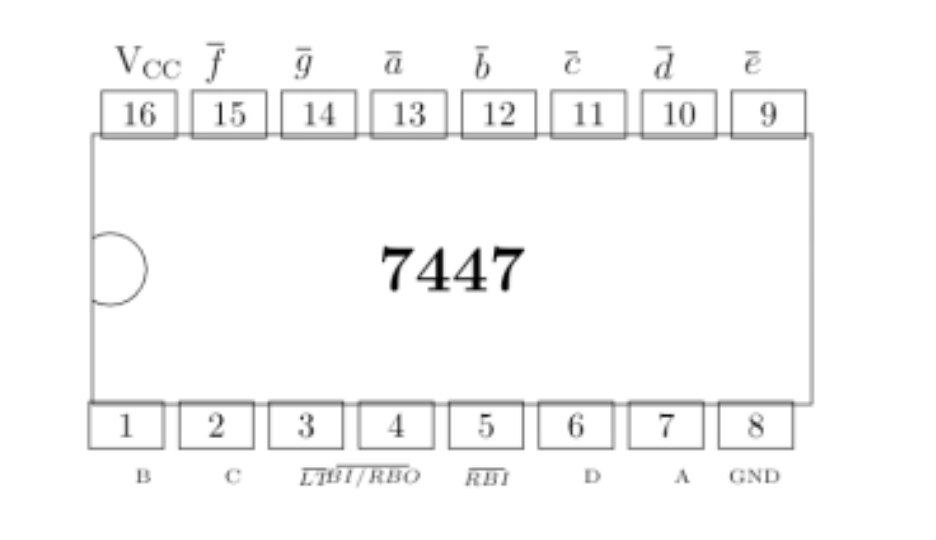
\includegraphics[width=\linewidth]{img/7447.jpg}
		\caption{ Decoder 7447}
		\label{fig-4}
	\end{figure}
	\begin{figure}[ht]
		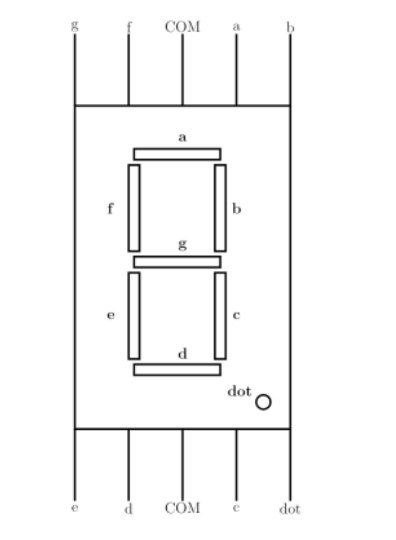
\includegraphics[width=\linewidth]{img/7-seg.jpg}
		\caption{7 segment display}
		\label{fig-5}
	\end{figure}
	\begin{figure}[ht]
		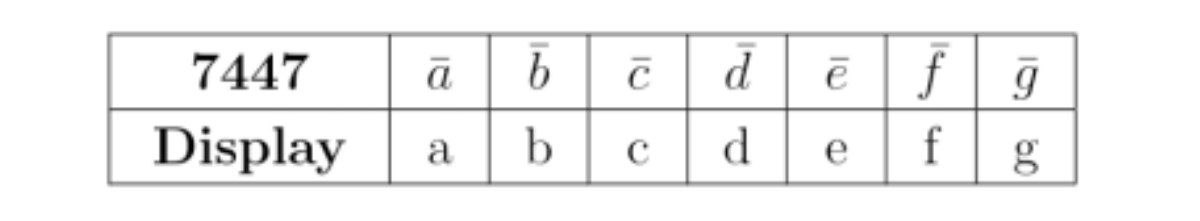
\includegraphics[width=\linewidth]{img/7447_table.jpg}
		\caption{ table}
		\label{fig-6}
	\end{figure}
	\begin{figure}[ht]
		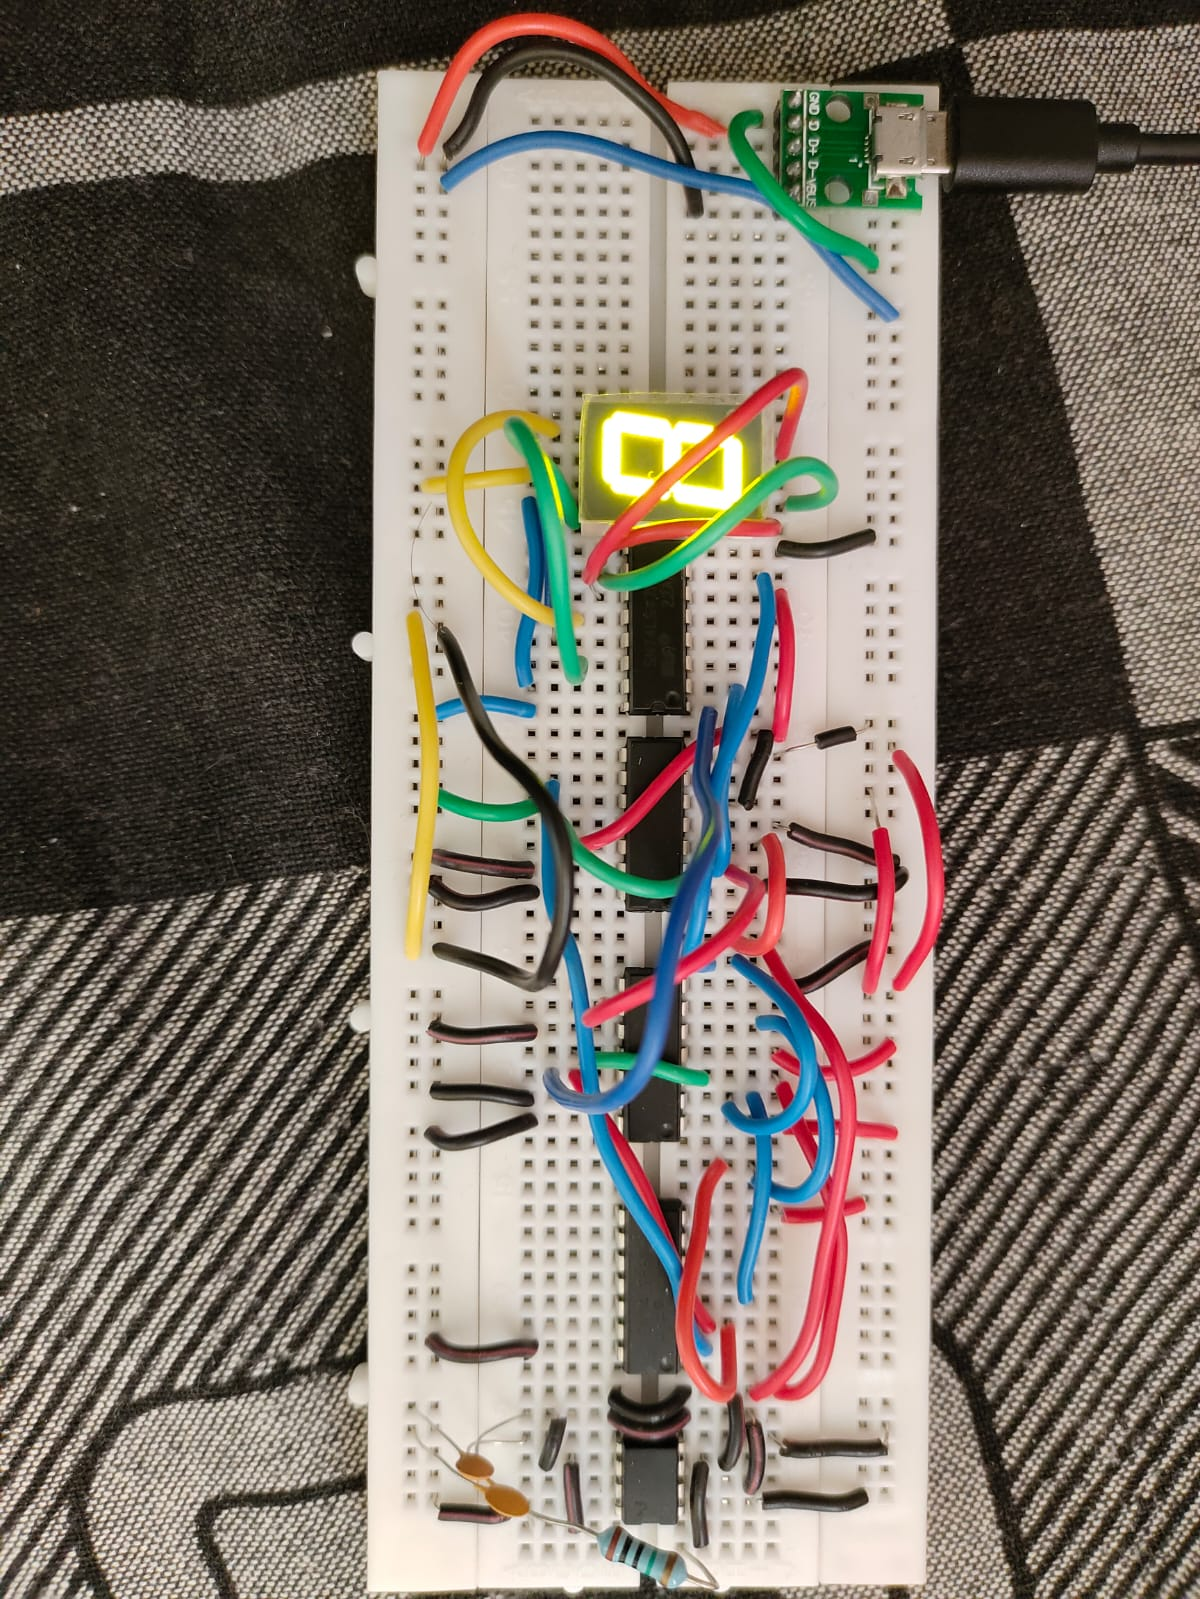
\includegraphics[width=\linewidth]{img/output.jpeg}
		\caption{output}
		\label{fig-7}
	\end{figure}




	
\end{document}
